\textit{This section was contributed by Ian Rose}.

Free surfaces are numerically challenging but can be useful for self consistently
tracking dynamic topography and may be quite important as a boundary condition
for tectonic processes like subduction. The parameter file \url{cookbooks/free_surface/free_surface.prm} 
provides a simple example of how to set up a model with a free surface, as well 
as demonstrates some of the challenges associated with doing so.

\aspect{} supports models with a free surface using an Arbitrary Lagrangian-Eulerian 
framework (see Section~\ref{sec:freesurface}). Most of this is done internally, so you do not need to worry about the
details to run this cookbook.  Here we demonstrate the evolution of surface topography 
that results when a blob of hot material rises in the mantle, pushing up the free
surface as it does.  Usually the amplitude of free surface topography 
will be small enough that it is difficult to see with the naked eye in visualizations,
but the \texttt{topography} postprocessor can help by outputting the maximum and minimum 
topography on the free surface at every time step. 

The bulk of the parameter file for this cookbook is similar to previous ones in this manual.
We use initial temperature conditions that set up a hot blob of rock in the center of the 
domain.

The main addition is the \texttt{Mesh deformation} subsection.
In this subsection you need to give \aspect{} a comma
separated list of the boundary indicators where the `free surface' deformation should be applied.
In this case, we are dealing with the `top' boundary of a box in 2D.
There is another significant parameter that needs to be set here: the value for the stabilization parameter ``theta''.
If this parameter is zero, then there is no stabilization, and you are likely to
see instabilities develop in the free surface. If this parameter is one then it
will do a good job of stabilizing the free surface, but it may overly damp its 
motions. The default value is 0.5.

Also worth mentioning is the change to the initial time step size. Stability concerns typically 
mean that when making a model with a free surface you will want to take smaller 
time steps. In general just how much smaller will depend on the problem at hand
as well as the desired accuracy. Because this model has a very smooth time evolution
it is sufficient to reduce the time step size of the first few time steps.

Following are the sections in the input file specific to this testcase.  The full parameter
file may be found at \url{cookbooks/free_surface/free_surface.prm}.

\lstinputlisting[language=prmfile]{cookbooks/free_surface/doc/free_surface.part.prm.out}

Running this input file will produce results like those in Figure~\ref{fig:freesurface}.
The model starts with a single hot blob of rock which rises in the domain.  As it 
rises, it pushes up the free surface in the middle, creating a topographic high there.
This is similar to the kind of dynamic topography that you might see above a mantle 
plume on Earth.  As the blob rises and diffuses, it loses the buoyancy to push up 
the boundary, and the surface begins to relax.

After running the cookbook, you may modify it in a number of ways:
\begin{itemize}
\item Add a more complicated initial temperature field to see how that affects topography.
\item Add a high-viscosity lithosphere to the top using a compositional field to tamp down on topography.
\item Explore different values for the stabilization theta and the CFL number to understand the nature of when and why stabilization is necessary.
\item Try a model in a different geometry, such as spherical shells.
\end{itemize}

\begin{figure}
  \centering
  
\includegraphics[height=0.25\textwidth]{cookbooks/free_surface/doc/free_surface_blob.png}
  \hfill
  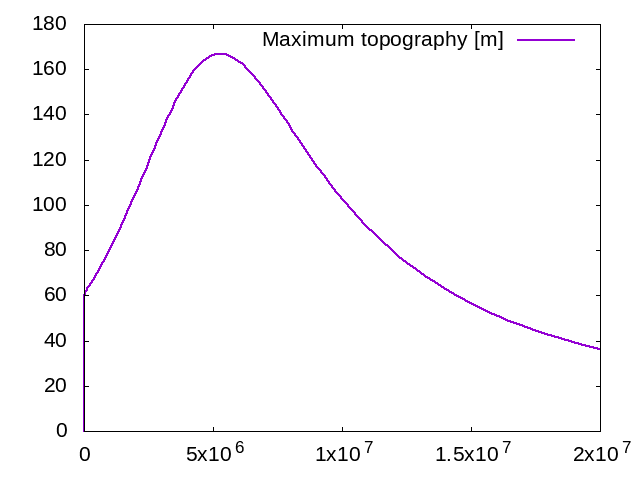
\includegraphics[height=0.25\textwidth]{cookbooks/free_surface/doc/free_surface_topography.png}
  \caption{\it Evolution of surface topography due to a rising blob.  On the left is a 
           snapshot of the model setup.  The right shows the value of the highest 
           topography in the domain over 18 Myr of model time.  The topography peaks
           at 167 meters after 5.5 Myr.  This cookbook may be run with the
           \url{cookbooks/free_surface/free_surface.prm} input file.}
  \label{fig:freesurface}
\end{figure}
